% ---
% titre: Fraction d'une quantité (représenter)
% theme: NO
% chapitre: Nombres rationnels
% sous_chapitre: Représenter, comparer et encadrer
% niveau: [10e]
% type: EVAL
% tags: [c-fractions, c-representer, p-question-TS]
% difficulte: 1
% corrige: true
% ---

\newcommand{\casquette}{%

\begin{tikzpicture}[scale=0.34,baseline=-0.25cm]

    % partie principale de la casquette
    \draw[very thick,rounded corners=2pt]
        (0,0)
        .. controls (0.1,0.9) and (0.7,1.35) .. (1.5,1.35)
        .. controls (2.2,1.35) and (2.7,0.9) .. (2.8,0.35)
        -- (1.2,0.35)
        .. controls (0.7,0.3) and (0.3,0.15) .. (0,0);

    % visière
    \draw[very thick]
        (1.2,0.35)
        .. controls (2.2,-0.15) and (3.1,-0.05) .. (3.5,0.25)
        .. controls (3.0,0.42) and (2.4,0.45) .. (2.8,0.35);

    % couture centrale
    \draw[thick]
        (1.5,1.35) -- (1.45,0.45);

    % petit bouton sur le dessus
    \fill (1.5,1.35) circle (0.07);

\end{tikzpicture}%
}

\question[3]
Colorie $\dfrac{3}{8}$ des casquettes. N'oublie pas de compléter la phrase.

\vspace{10pt}
Je divise les casquettes en \sol{\;\bl\;}{8} groupes. \quad Je colorie les casquettes de \sol{\;\bl\;}{3} groupes.\\[6pt]

\begin{center}
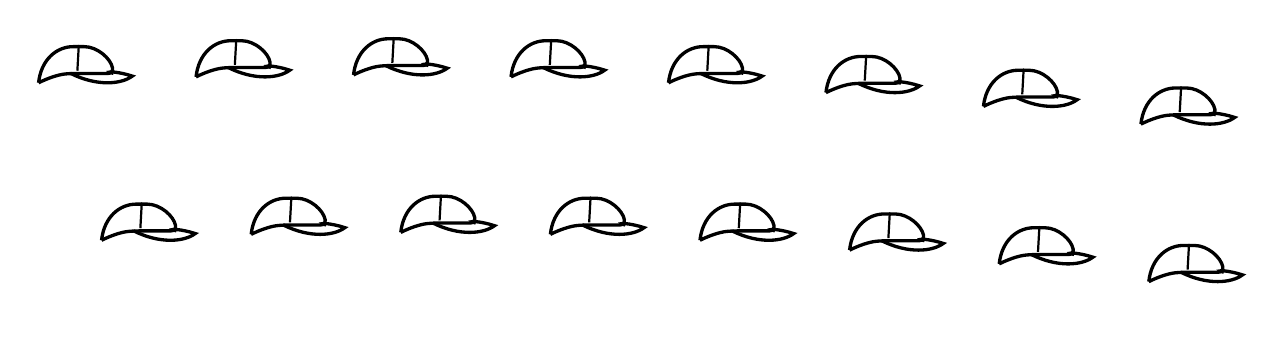
\begin{tikzpicture}
\foreach \i in {0,...,7}{\node at (\i*2,0.1*\i-0.1*\i*\i/4) {\casquette};}
\foreach \i in {0,...,7}{\node at (\i*1.9+0.8,-2+0.1*\i-0.1*\i*\i/4) {\casquette};}
\end{tikzpicture}
\end{center}


\begin{solution}[0pt]
\textbf{1\,pt} pour le nombre de groupes, \textbf{1\,pt} si tous les groupes sont égaux, \textbf{1\,pt} pour les casquettes coloriées.\\[4pt]
$16$ casquettes en $8$ groupes de $2$ : $3$ groupes coloriés, soit $6$ casquettes.
\end{solution}